%!TEX TS-program = xelatex
%!TEX encoding = UTF-8 Unicode

\title{
    \Large Fish-eye transformation with bilinear interpolation \\
    \large CS-425 Program parallelization on PC clusters}
\author{
    Yoan Blanc \texttt{yoan.blanc@epfl.ch}
}
\date{\today}

\documentclass[10pt,a4paper]{article}
\usepackage{amsfonts}
\usepackage{amsmath}
\usepackage[svgnames]{xcolor}
\usepackage{graphicx}
\usepackage{hyperref}
\usepackage{url}
\usepackage{verbatim}
\usepackage{fontspec}
\usepackage{tikz}
\usepackage{framed}
\setmainfont[Mapping=tex-text,Ligatures={Common,Rare,Discretionary}]{Linux Libertine O}
\newfontfamily\quotefont[Mapping=tex-text,Ligatures={Common,Rare,Discretionary}]{Linux Libertine O}

% http://tex.stackexchange.com/questions/16964/block-quote-with-big-quotation-marks
% Make commands for the quotes
\newcommand*{\openquote}{\tikz[remember picture,overlay,xshift=-15pt,yshift=-10pt]
\node (OQ) {\quotefont\fontsize{60}{60}\selectfont``};\kern0pt}
\newcommand*{\closequote}{\tikz[remember picture,overlay,xshift=15pt,yshift=10pt]
\node (CQ) {\quotefont\fontsize{60}{60}\selectfont''};}
% select a colour for the shading
\definecolor{shadecolor}{named}{Azure}
% wrap everything in its own environment
\newenvironment{shadequote}%
{\begin{snugshade}\begin{quote}\openquote}
{\hfill\closequote\end{quote}\end{snugshade}}

\begin{document}
\maketitle

\section{Abstract}
\textbf{TODO}

\section{Description}
% A brief description of the application and its computational complexity
% (O(n), O(nlogn), ...). Provide an upper bound of the achievable speedup using
% Amdahl’s law.

The fish-eye transformation with a bilinear interpolation works as such: for
each pixel in the destination picture, look at what the lens sees in the
source picture and compute its value by interpolating the potentially four
surrounding pixels.

\subsection{Computational complexity}

Let $(x, y)$ by the pixel coordinate (Cartesian system), $(r, \theta)$ the
pixel coordinate (polar system), $(w, h)$ the picture geometry, $m$ the
magnification factor and $R$ the radius of the applied lens. $(x\prime,
y\prime)$ and $(r\prime, \theta\prime)$ are the pixels in the source picture.
And $v(x,y)$ represents the red-green-blue value in the destination picture
while $v\prime(x,y)$ is this value in the source picture.

The algorithm works as follow:

\begin{itemize}
    \item for each pixel in the destination picture, convert their position
    into the polar coordinates to see if it belongs to the lens.

    $r = \sqrt{(\frac{w}{2}-x)^2 + (\frac{h}{2}-y)^2}$

    if $r < R$ then it must be magnify, otherwise simply take the same pixel
    from the source picture.

    \item Now that it's part of the magnified part, we have to compute the
    $\theta$ value to apply the magnification factor $m$ to it.

    $$\theta = atan2(\frac{h}{2} - y, \frac{w}{2} - x)$$

    The angle is not affected by the lens, thus: $\theta\prime = \theta$.

    $$r\prime = \frac{1}{1 + m\frac{1-r}{r}}$$

    At this point, we have $(r\prime, \theta\prime)$ and have to go back to
    Cartesian coordinates to obtain: $(x\prime, y\prime)$ using the reverse
    formula from above.

    \item If $x$ and $y$ are in $\mathbb{N}$, $x\prime$ and $y\prime$ are in
    $\mathbb{Z}$, we must then perform the value interpolation. A simple
    rounding operation would produce a clumsy output. If rounding would
    consider $1$ pixel, the bilinear interpolation uses all $4$ surrounding
    ones.

    \begin{align}
    dx &= x\prime - \lfloor{}x\prime\rfloor{} \\
    dy &= y\prime - \lfloor{}y\prime\rfloor{}
    \end{align}

    The small $x$-offset and $y$-offset are the ratio applied to each of the
    $4$ considered pixels.

    \begin{align*}
    v(x, y) =
    (1-dy) &\cdot \big(
        (1-dx) \cdot v\prime(\lfloor{}x\prime\rfloor{},\lfloor{}y\prime\rfloor{}) +
        dx \cdot v\prime(\lceil{}x\prime\rceil{},\lfloor{}y\prime\rfloor{})
    \big) + \\
    dy &\cdot \big(
        (1-dx) \cdot v\prime(\lfloor{}x\prime\rfloor{},\lceil{}y\prime\rceil{}) +
        dx \cdot v\prime(\lceil{}x\prime\rceil{},\lceil{}y\prime\rceil{})
    \big)
    \end{align*}

\end{itemize}

The algorithm iterates over the pixels and may read up to 4 times the source
pixels. It's worst case complexity is $O(4n)$, which is linear: $O(n)$ where
$n$ is the size of the source picture in pixels.

\subsection{Theoretical speed-up}

The algorithm's simplicity makes it totally parallelizable if we assume that
the destination picture resides at a different memory space than the source
picture. Each destination pixel can be calculated independently of the others.
This algorithm has no serial parts in it.

Using \emph{Amdahl's law}, we can conclude that $S(N) = N$, a perfect speedup
could be achievable if we ignore all \emph{input/output} considerations.

\section{Parallelization strategies}
% Define different parallelization strategies, and describe the pros and cons
% of each one of them. Compute their respective communication complexities, as
% well the computation to communication ratio.
Two parallelization strategies will be explored, shared memory using OpenMP and
message passing with MPI. OpenMP is quite straightforward, while MPI will
require to split the destination picture in parts that will be distributed and
gathered by one master node, combining and saving the destination picture.

\subsection{MPI}
%  b. If you use MPI, draw a message-passing graph that describes your
%     implementation, and specify the content of the transferred messages.
Each nodes will open the source file, compute one part of it: an horizontal
slice and send it to the node $0$ that will merge them into the final picture.

The node $0$ will compute one slice and copy other the destination picture the
border outside the lens area. All other nodes will compute a slice and send it
to the node $0$. Other nodes could compute more than one slice taking
advantages of the asynchronous send operations to start computing the next
part (see: \emph{Figure \ref{fig:slices}}).

\begin{figure}[h]
    \centering
    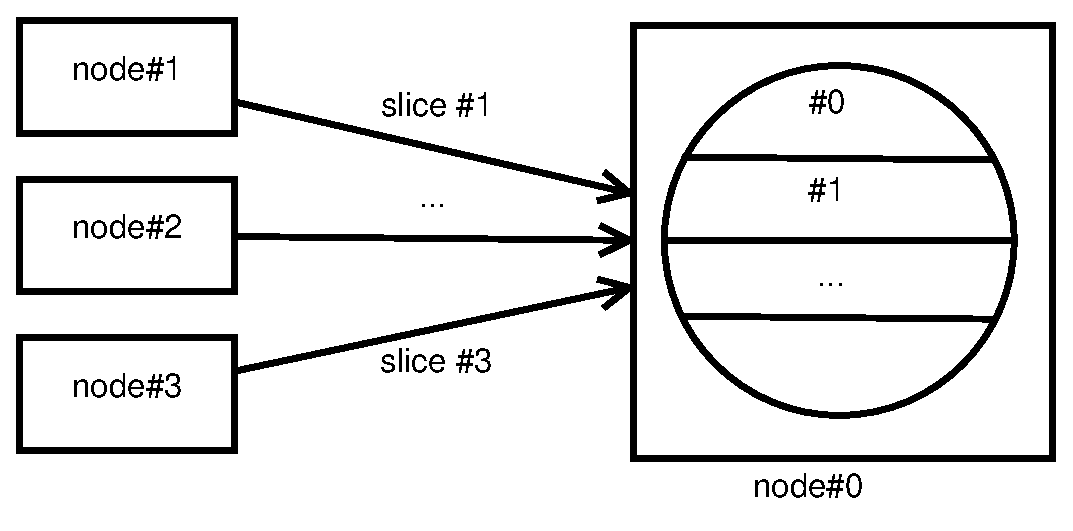
\includegraphics[width=0.5\linewidth]{../figures/slices.eps}
    \caption{Messages passing}{\small Each node other than $0$ will send its
    slice to node $0$, a slice is an horizontal and rectangular chunk of the
    area where the lens is applied to.}
    \label{fig:slices}
\end{figure}

\subsection{OpenMP}
%  c. If you use OpenMP or a GPU (CUDA), describe the flow of your program as a
%     sequence of serial and parallel sections, possibly with the type of chunk
%     decomposition and scheduling used.
The shared memory implementation will add one part to the algorithm:
\textbf{precomputation of the lens} (find more under the section \emph{Possible
optimizations}). And thus have two serial parts, reading and writing the file
as well as two parallel sections: precomputation of the lens, magnification of
the picture. Both sections are working on independent pixels and can be
totally parallelized.

\section{Theoretical Analysis}
% Provide a detailed theoretical analysis of one or more of your strategies
% using a timing diagram taking into account the computing and communication
% times, the pipelining of operations, etc.  From the critical path, derive a
% theoretical model enabling predicting the speedup of the application on an
% arbitrary number of machines.  Some applications may have data dependent
% behaviors preventing a general theoretical model from being derived. In such
% cases, choose one or two inputs and derive a model for these particular
% cases. Compare the results with your initial guess using Amdahl’s law.

\subsection{MPI}

A speedup can only be achieved if the size of the data to send over the wire is
takes less time to send than to compute. The timing diagram (see: \emph{Figure
\ref{fig:mpi}}) assumes that and also assumes that the recieving time outgrows
the time to copy the data back into the destination file so this operation can
be done will more data is recieved (by buffering).

\begin{figure}[h]
    \centering
    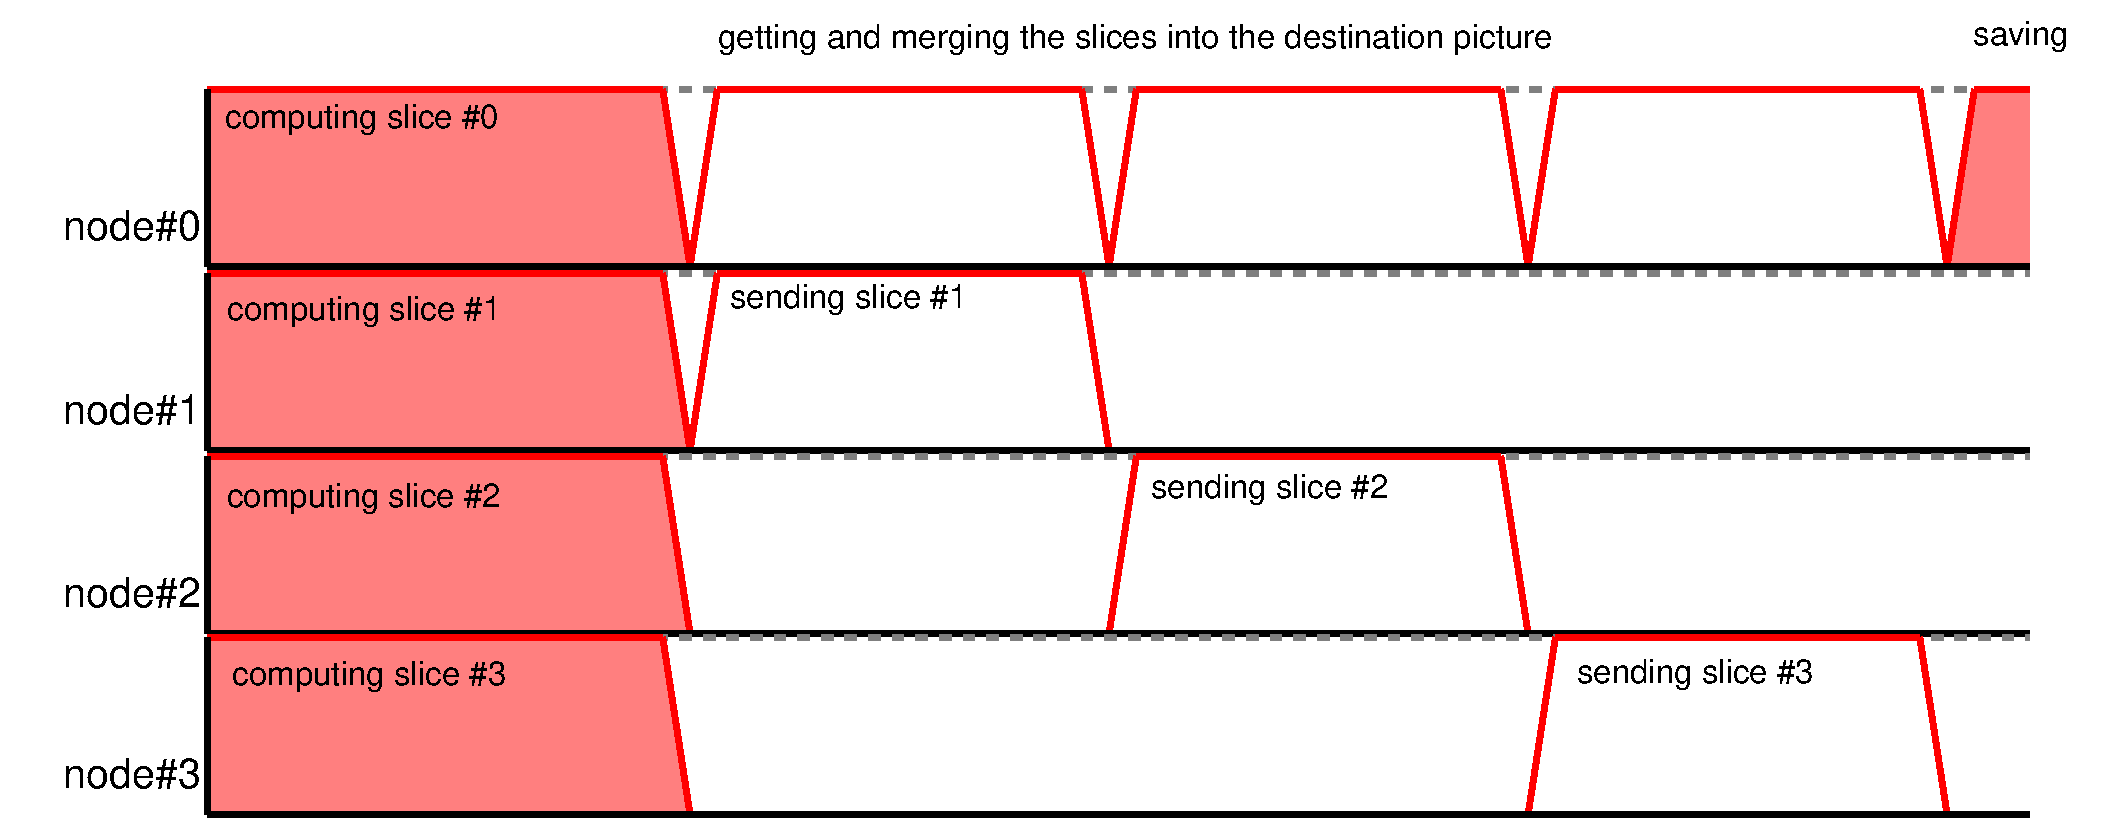
\includegraphics[width=0.9\linewidth]{../figures/mpi.eps}
    \caption{Messages passing timing diagram}{\small Every node compute a slice
    (or chunk) of the picture, sends it to the master node which will combine
    them and produce the output picture.}
    \label{fig:mpi}
\end{figure}

\subsubsection{Computation vs communication}
Assuming a 8000x8000x24bits bitmap picture. Measures were done in the INF3 room
at the EPFL.

\begin{itemize}
    \item Picture size (lens area only): $7200^2 \cdot 3 = 148 MB$
    \item Bandwidth: $9.7 MB/s$, latency: $5.75 ms$
    \item Computational time: $18 sec$
    \item Communication time: $\frac{148}{9.7} = 15 sec$
\end{itemize}

$$Ratio = \frac{18}{15} = 1.2$$

\subsubsection{Speedup}

We can get a small $20\%$ improvement of getting something from the network
rather than computing it ourself. Scaling this to $n$ nodes, it gives us the
following formula.

$$t_{parallel}(n) = \frac{t_{linear}}{n}(1 + \frac{n - 1}{1.2})$$

\begin{align*}
speedup(n) &= \frac{t_{linear}}{t_{parallel}} \\
        &= \frac{t_{linear}}{\frac{t_{linear}}{n}(1 + \frac{n - 1}{1.2})} \\
        &= \frac{n}{1 + \frac{n - 1}{1.2}} \\
        &= \frac{1.2}{1 + \frac{0.2}{n}}
\end{align*}

The speed up increases with $n$, slowly and will top at $1.2$.

\subsection{OpenMP}
Same as the initial guess using \emph{Amdahl's law}. We can achieve a perfect
speedup if we don't consider I/O.

\subsection{Possible optimizations}
% If applicable, discuss possible optimizations of the parallel implementation
% and of the algorithm.
The lens has a central symmetry if we only consider the new position's offsets
and not the source picture. Hence, a matrix of $\frac{1}{4}$ of the total lens
can be precomputed and reused for every quadrants of the picture.

\begin{figure}[h]
    \centering
    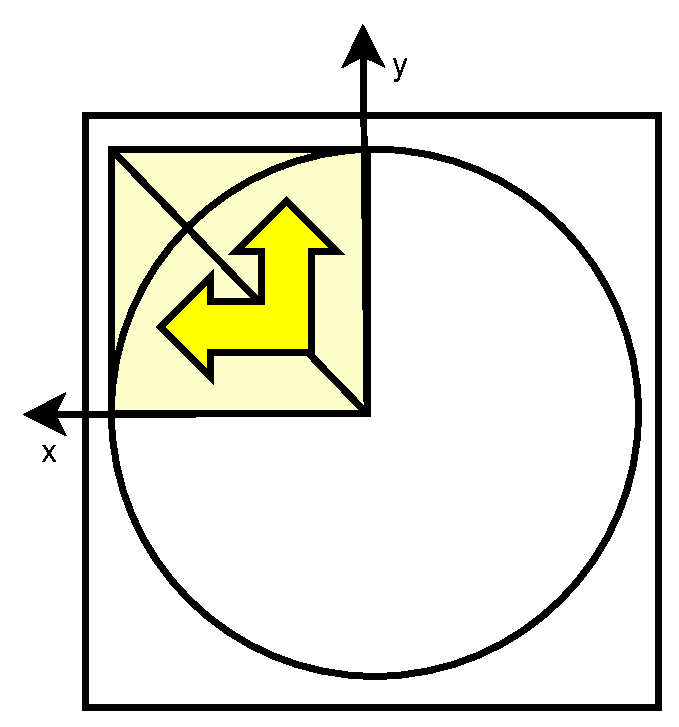
\includegraphics[width=0.3\linewidth]{../figures/lens.eps}
    \caption{Lens precomputation}{The top left hand corder vectors are stored
    in memory but only the first eighth is effectively computed, the other one
    is obtained by symmetry.}
    \label{fig:lens}
\end{figure}

This matrix contains the relative position of the source pixel from the
destination pixel.  In other words, we record the difference between the two
vectors.

\begin{align*}
lens_{x,y}
    &= \left(\! \begin{array}{c} l_x \\ l_y \end{array} \!\right) \\
    &= \left(\! \begin{array}{c} x \\ y \end{array} \!\right)
    - \left(\! \begin{array}{c} x\prime \\ y\prime \end{array} \!\right)
\end{align*}

For each quadrants, it's easy to compute back its vector:

\begin{itemize}
    \item Top left: $\left(\! \begin{array}{c} l_x \\ l_y \end{array}
    \!\right)$

    \item Top right: $\left(\! \begin{array}{c} -l_x \\ l_y \end{array}
    \!\right)$

    \item Bottom left: $\left(\! \begin{array}{c} l_x \\ -l_y \end{array}
    \!\right)$

    \item Bottom right: $\left(\! \begin{array}{c} -l_x \\ -l_y \end{array}
    \!\right)$

\end{itemize}

This optimization makes sense if:

\begin{itemize}
    \item the program can share the lens (shared memory) or
    \item if the nodes have to compute more than one eighth of the final
    picture, otherwise it'll precompute more than required and waste resources.

\end{itemize}

\section{Implementations}
% Depending on the complexity of the application, implement one or several of
% the described strategies, and describe the related issues.

\begin{shadequote}
    FIRST OPTIMIZE ON ONE CORE, THEN PARALLELIZE (the right
    algorithm) \\ ---\emph{Vincent Keller}
\end{shadequote}

\subsection{Serial versions}
As a matter of fact, I did many serial versions, spending a lot a time trying
to improve the \emph{input/output} time which was told to me during the
presentation that I shouldn't have. Nonetheless, I'll present them and they
have an impact on the shared memory solution.

\begin{itemize}
    \item \textbf{Serial 0}\\
    One naive version using ``ray tracing'' (going from destination to source)

    \item \textbf{Serial 1} ~(computational)\\
    \emph{Serial 0} + the naive version with pre-calculated rays optimization.

    \item \textbf{Serial 2} ~(computational)\\
    \emph{Serial 1} + the pre-calculated optimization for the fish-eye (lens)
    zone only.

    \item \textbf{Serial 3} ~(memory, computational)\\
    \emph{Serial 2} + making the transformation in place plus some
    computation optimizations (\verb|for-loops|)

    \item \textbf{Serial 4} ~(memory)\\
    \emph{Serial 3} + use a smaller mask, only $\frac{1}{4}$ of the full lens.

    \item \textbf{Serial 5} ~(I/O)\\
    \emph{Serial 4} + Opening the source file using \texttt{mmap}
    (\verb|MMAP(2)|) and not working in-place anymore.

    \item \textbf{Serial 6} ~(memory, I/O)\\
    \emph{Serial 4} + Copying the source file to destination using
    \texttt{sendfile} (\verb|SENDFILE(2)|), working in place and using
    \texttt{mmap} \end{itemize}.

\subsubsection{Serial 0}

The naive serial version works as explained in the analysis section.

\subsubsection{Serial 1}

This improvement does the very same as serial 0 but will make $25\%$ less polar
to radius calculation by pre-calculating the $(x\prime,y\prime)$ values for
each pixel. The fisheye mask as a central symmetry. So it exploits it to only
calculate the top left quarter of the picture and then transpose it to the $3$
others. Now while building the destination picture, the source pixel is
obtained by using the mask (the solid arrow) instead of calculating everything
(the dashed arrow).  The billinear interpolation (the dotted arrow) still needs
to be done since there are no assumed symmetric in the source picture.

\subsubsection{Serial 2}

It’s building upon \emph{Serial 1}, with a little improvement. The mask is not
only symmetrical in $4$ but in $8$ as well easily if the mask is a square. And
as everything outside the fisheye lense is set to null, it’s simply wasted
space. In face, the mask is infinity-symmetrical but it gets tricky in
cartesian coordinates (but doable still if the mask’s size are okay). Here it
does less calculation and uses less storage for the mask.

\subsubsection{Serial 3}

Building from \emph{Serial 2}, it removes the need of having a source and a
destination and works in the source data directly. It wasn’t possible because
while read from top to bottom and left to right, everything but the top left
corner will modify data it’ll read later on. The algorithm here will act
differently for each quarter of the output picture. And other gain, everything
from the source picture outside the lens don’t have to be copied over to the
destination one.

\subsubsection{Serial 4}

Same as with \emph{Serial 3} but stores only $\frac{1}{4}$ of the mask. This is
the optimization described in the analysis section.

\subsubsection{Serial 5}

Built from \emph{Serial 4}, it uses \verb|mmap| to load the file cutting down
the \emph{input/output} time. This solution only works on GNU/Linux and has to
be ported to MS Windows if required. Compared to \emph{Serial 4}, this solution
cannot work in place anymore as the loaded picture lives in the same memory
space as the real one, on disk.

\subsubsection{Serial 6}

Just like \emph{Serial 5} but works in place by copying the source picture to
the destination one using \verb|sendfile|, then loading it using \verb|mmap|
and finally working in place.

It doesn't seem to bring much on the speed side. Memory wise it has only the
lens (on the heap) and the destination picture loaded.

\subsection{MPI versions}
Three versions has been made, the first two ones ($0$ and $1$) were done before
the project presentation and thus tried to minimized load time as well.

\subsubsection{MPI 0}

This version parallelize the lens pre-computation with the source image opening.

\subsubsection{MPI 1}

This second version opens the source file at the root node, sends it to the all
the workers in chunks (the 4 quadrants) while they all are pre-computing the
lens.

The picture is send two times (back and forth) over the network which is less
than optimal.

\subsubsection{MPI 2}

This version is very implementation of the algorithm described in the analysis
part. The source picture is opened by each node, they all compute one chunk of
the final picture and send it to the main node.

\subsection{OpenMP versions}

\subsubsection{OpenMP 0}

This version is built from \emph{Serial 4} and tries to cut I/O time by
precomputing the lens while the source file is read. Sadly the memory bandwidth
appears to be make the reading of the file way slower than it used to be.

\subsubsection{OpenMP 1}

That second version is built from \emph{Serial 5}. Both the lens precomputation
and the lens application are done in parallel dynamic schedules.

\section{Evaluations}
% Evaluate the performance of the application on at least 1, 2, 4 and 8 nodes.
% Draw a speedup graph combining the practical absolute (in respect to a serial
% execution), relative (in respect to a parallel execution on a single node)
% and theoretical speedup, as well as Amdahl’s law. Mention the reference
% execution time. Discuss any difference between your original prediction and
% the actual results and provide a corrected model if needed. If applicable,
% compare practical results for different types of sizes of inputs, the impact
% of the different optimizations, etc.

\section{Conclusion}
\textbf{TODO}

%\bibliographystyle{unsrt}
%\bibliography{report}

\end{document}
